\chapter{Multilanguage queries}
\label{chap:multilang-queries}

In DortDB, we want to provide a common framework for queries regardless of the query language. A direct conclusion is to allow mixing languages in a single query. This enables the user to separate their query into logical parts and express each in a language they find the most intuitive. It also offers the possibility to form multimodel queries using the languages initially developed for each model.

Existing implementations of this idea include SQL/XML or OpenLink Virtuoso's SPASQL\cite{virtuoso_spasql}. SQL/XML uses new functions and datatypes, which facilitate queries combining relational and document models, but it is rather verbose. SPASQL, or SPARQL-in-SQL, allows for embedding SPARQL subqueries into SQL. However, it is not possible to embed SQL subqueries into SPARQL.

\section{Language switching}
\begin{comment}
- dict X single value
- arango db: forin
- orient db: no join
- spasql: rel X rel

Algebra:

- https://ieeexplore.ieee.org/abstract/document/1617382 (xquery)
- https://ieeexplore.ieee.org/abstract/document/1410186 (xpath)
- Optimization of Nested Queries using the NF2 Algebra
- Handling Environments in a Nested Relational Algebra
with Combinators and an Implementation in a Verified
Query Compiler
- SQL query optimization through nested relational algebra
- The relational model with relation-valued attributes
- https://arxiv.org/pdf/2407.04823
- https://arxiv.org/pdf/1908.06265v1
- https://drops.dagstuhl.de/storage/00lipics/lipics-vol098-icdt2018/LIPIcs.ICDT.2018.9/LIPIcs.ICDT.2018.9.pdf
- https://cseweb.ucsd.edu/classes/wi20/cse232B-a/papers/staircase.pdf
\end{comment}

Our approach extrapolates on SPASQL to allow embedding any language subqueries into any language. It is necessary to establish clear rules for the language-to-language interfaces. In some cases, the transition is intuitive -- e.g., a SQL query that selects attributes from a Cypher subquery. The Cypher subquery returns a set of tuples, just like a SQL subquery would. On the other hand, SQL might sometimes require the subquery only to produce a single value. Some languages do not operate in terms of tuples, such as XPath. Our solution is to separate the subqueries into those producing tuples and those producing opaque items. Each language is then responsible for converting the results of these subqueries as necessary.

\begin{listing}[!ht]
\begin{minted}{sql}
SELECT attr1, attr2 FROM (
  -- subquery
);

SELECT (SELECT count(*) FROM table1) AS total, count(*)
FROM table1
GROUP BY item_id;
\end{minted}
\caption{Example of two SQL subqueries. The first subquery produces tuples, the second produces only a single value.}
\end{listing}

The language switch subqueries are demarcated by the \texttt{LANG} keyword on one side and either by a scope exit (a closing bracket or parenthesis) or by the \texttt{LANG EXIT} keywords on the other. The nested language can use variables available in the parent scope. In case of languages such as SQL, the attributes used by the nested language are used to infer the schema of referenced relations.

\begin{listing}[!ht]
\begin{minted}{sql}
SELECT id, ARRAY(
  LANG cypher
\end{minted}
\nestedMintedVspace
\begin{minted}[style=manni]{cypher}
  MATCH (:person {id: people.id})-[:KNOWS]->(friend)
  RETURN friend
\end{minted}
\nestedMintedVspace
\begin{minted}{sql}
) AS friends
FROM people
\end{minted}
\caption{Cypher nested into SQL refers to the outer relation \texttt{people}.}
\end{listing}

\begin{figure}[htpb]
    \begin{subfigure}[b]{\textwidth}
    \begin{tcolorbox}[colback=white, colframe=black, boxrule=1pt, arc=0pt]
        \begin{minted}[fontsize=\small]{sql}
SELECT foo.frst, (
  LANG xquery
        \end{minted}
        \nestedMintedVspace
        \begin{minted}[style=manni,fontsize=\small]{xquery}
  for $x in $xs
  return $foo:second + (
        \end{minted}
        \nestedMintedVspace
        \begin{minted}[fontsize=\small]{sql}
    LANG §\texttt{sql}§
    SELECT foo.third FROM bar
  )
) AS nested
FROM foo
        \end{minted}
    \end{tcolorbox}
    \end{subfigure}
    
    \medskip
    
    \begin{subfigure}[b]{\textwidth}
        \centering
        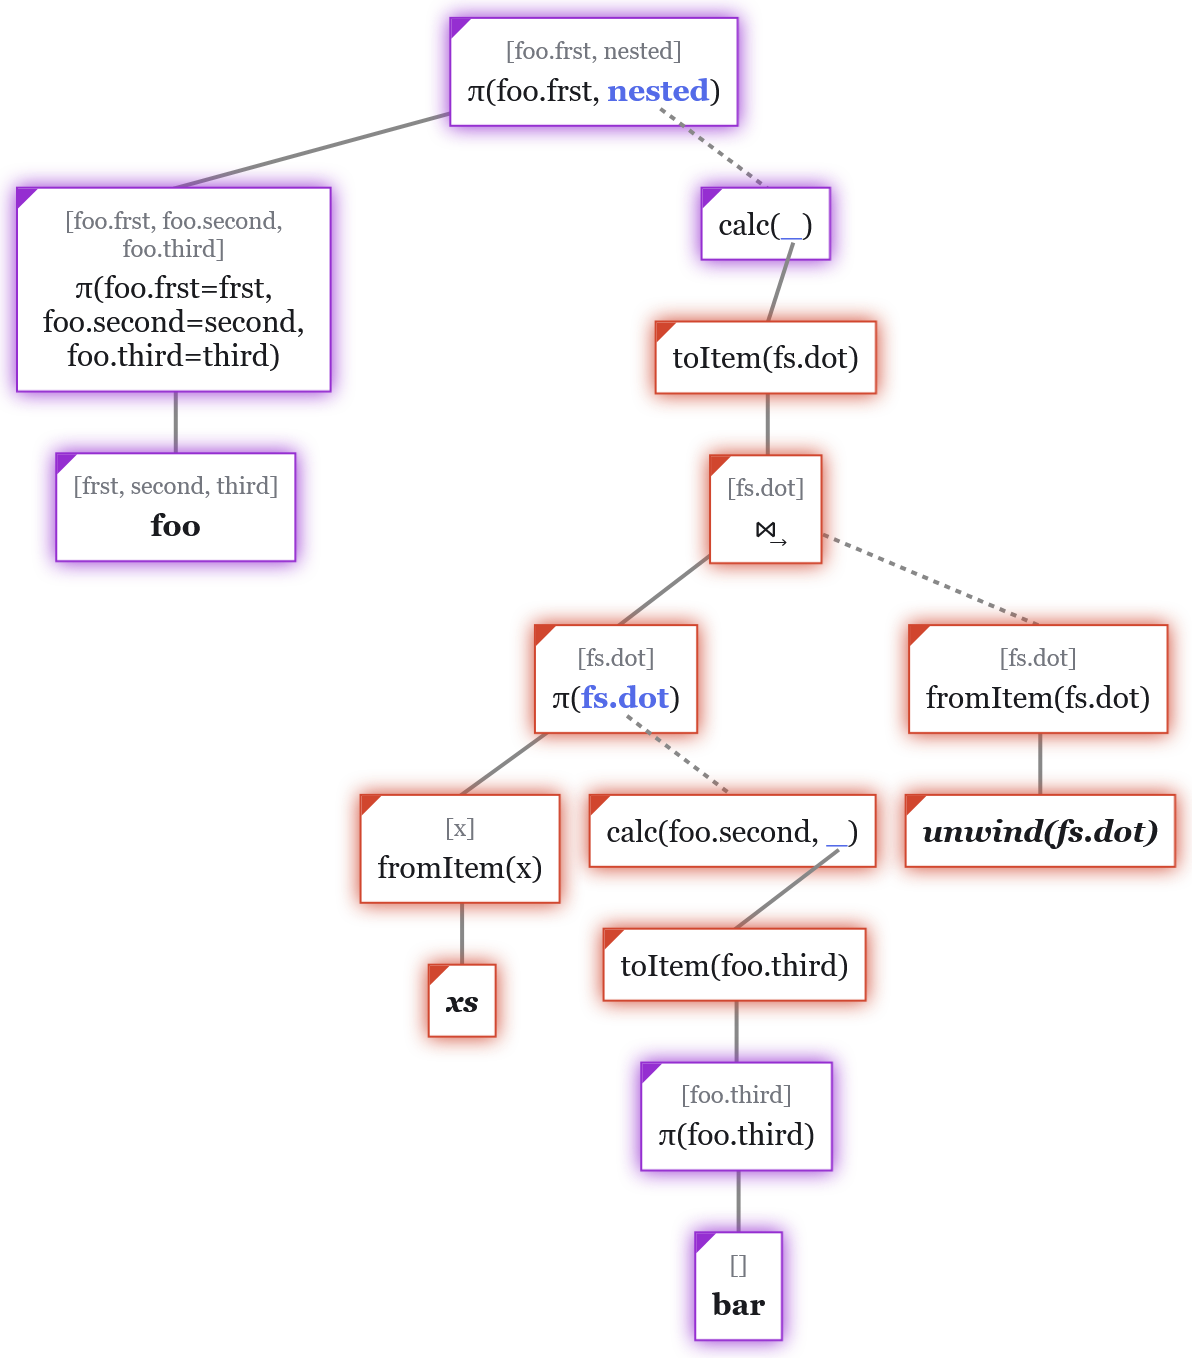
\includegraphics[width=360pt]{img/tree-sql-infer.png}
    \end{subfigure}
    
    \caption{The SQL parser can use information from the nested languages to infer the schema of the \texttt{foo} relation. The logical operator tree is partially optimized for better readability. Diagrams like this are explained in section \ref{sec:algebra}. For now, the important thing is that the grey brackets in some nodes denote the tuple schema of the corresponding operator.}
\end{figure}

\section{Unified algebra}
\label{sec:algebra}

Queries are parsed into a logical operator tree, where each node corresponds to an operator from \textit{unified algebra}. The unified algebra covers most of the expected query operations. It is, however, possible for any language to extend the algebra and to define its own operators. This way, it is possible to cover any future languages regardless of their model. This process is more closely explained in section \ref{sec:usage-extensibility}.
%\hl{/*KOP je/bude nekde popsane, jak to udelat? (Cestina s hacky a carkami se v PDF spatne renderuje, tak budu psat komentare bez nich.)*/}

%\hl{/*KOP z ciste estetickeho hlediska bych psal vsechny LANG jednotne velkymi pismeny. V obrazku je LANG xquery, ale lang sql.*/}

The algebra is based on algebras for XQuery\cite{xquery_algebra}, graph paths\cite{angles2024path} and nested relational algebra\cite{schek1986relational}. We divide the operators into two main groups. \textit{Tuple operators} operate on streams of named tuples, similarly to relational algebra. \textit{Item operators} operate on streams of opaque items. Depending on their arguments, some operators may be considered either item or tuple operators. One such example is the \texttt{limit} operator.

\begin{longtable}{|>{\raggedright\arraybackslash}p{5cm}|>{\raggedright\arraybackslash}p{9cm}|}
\hline
\textbf{Algebraic Operator} & \textbf{Operator's Signature} \\ 
\hline
\endfirsthead
\hline
\textbf{Algebraic Operator} & \textbf{Operator's Signature} \\ 
\hline
\endhead
\hline
\endfoot

\multicolumn{2}{|c|}{\textbf{Item Operators}} \\ 
\hline
\textbf{Calculation Intermediaries} & \\
AggregateCall & $\text{agg}(\texttt{args})$ \\
Conditional & $\text{cond}(\texttt{expr}, \texttt{whenthens}, \texttt{default})$ \\
FnCall & $\text{fn}(\texttt{args})$ \\
Literal & $\text{literal}(\texttt{value})$ \\
Quantifier & $\text{quant}(\texttt{type}, \texttt{query})$ \\
\hline
\textbf{Other} & \\
Calculation & $\text{calc}(\texttt{args})$ \\
ItemSource & $\textit{name}$ \\
ItemFnSource & $\textit{name}(\texttt{params})$ \\
MapToItem & $\text{toItem}(\texttt{key}, \texttt{source})$ \\
\hline
\multicolumn{2}{|c|}{\textbf{Tuple Operators}} \\ 
\hline
\textbf{SPJ} & \\
CartesianProduct & $\times(\texttt{left},\texttt{right})$ \\
Join & $\bowtie(\texttt{left},\texttt{right},$ $\texttt{leftOuter},\texttt{rightOuter},\texttt{conditions})$ \\
Projection & $\pi(\texttt{attrs},\texttt{source})$ \\
ProjectionConcat & $\stackrel{\bowtie}{\rightarrow}(\texttt{mapping}, \texttt{outer}, \texttt{source})$ \\
ProjectionIndex & $\text{index}(\texttt{name}, \texttt{source})$ \\
Selection & $\sigma(\texttt{expression}, \texttt{source})$ \\
\hline
\textbf{Other} & \\
Distinct & $\delta(\texttt{attributes}, \texttt{source})$ \\
GroupBy & $\gamma(\texttt{keys},\texttt{aggs},\texttt{source})$ \\
MapFromItem & $\text{fromItem}(\texttt{key}, \texttt{source}) $ \\
OrderBy & $\tau(\texttt{orders},\texttt{source})$ \\
Recursion & $\phi(\texttt{min}, \texttt{max}, \texttt{condition}, \texttt{source})$ \\
TupleSource & $\textbf{name}$ \\
TupleFnSource & $\textbf{name}(\texttt{params})$ \\
\hline
\textbf{XQuery} & \\
ProjectionSize & $\text{size}(\texttt{name}, \texttt{source})$ \\
TreeJoin & $\text{treeJoin}(\texttt{expr}, \texttt{source})$ \\
\hline
\textbf{Optimizer} & \\
IndexScan & $\textbf{indexScan}(\texttt{name}, \texttt{access})$ \\
IndexedRecursion & $\stackrel{\phi}{\rightarrow}(\texttt{min}, \texttt{max}, \texttt{mapping}, \texttt{source})$ \\
\hline
\multicolumn{2}{|c|}{\textbf{Universal Operators}} \\ 
\hline
NullSource & $\square$ \\
Limit & $\text{limit}(\texttt{skip}, \texttt{limit})$ \\
\hline
\textbf{Set} & \\
Difference & $\setminus(\texttt{left}, \texttt{right})$ \\
Intersection & $\cap(\texttt{left}, \texttt{right})$ \\
Union & $\cup(\texttt{left}, \texttt{right})$ \\
\hline

\end{longtable}

\subsection{Visualization}

The DortDB GUI includes visualization of query plans. The plans are visualized as a tree where each node corresponds to an operator. The tree's root is the final query; the leaves are individual data sources. Each node is colored based on the language it originated from. Tuple operator nodes include the operator schema. The edges are either a solid or a dashed line. Solid edges mean that the child operator is created only once at the same time as its parent. Dashed edges indicate a child operator that is dynamically recreated multiple times during its parent's lifetime.

The source code of the GUI is available as an appendix to this work. The GUI is also available online at \url{https://filipjezek.github.io/dortdb}. The reader is encouraged to try things out for themselves.

\begin{figure}[htpb]
    \begin{subfigure}[b]{\textwidth}
    \begin{tcolorbox}[colback=white, colframe=black, boxrule=1pt, arc=0pt]
        \begin{minted}[fontsize=\small]{sql}
SELECT x + 3 AS xplusthree FROM table1
        \end{minted}
    \end{tcolorbox}
    \end{subfigure}
    
    \medskip
    
    \begin{subfigure}[b]{\textwidth}
        \centering
        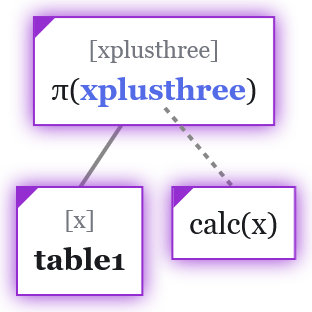
\includegraphics[width=90pt]{img/tree-edge-types.png}
    \end{subfigure}
    
    \caption{The different edge types: \texttt{tupleSource} \textbf{table1} is created once while the \texttt{calculation} is reevaluated for each source row. The \texttt{calculation} edge points directly to its blue representative attribute.}
\end{figure}

\subsection{Operators}

Most of the item operators are calculation intermediaries. They do not participate in the final query plan. Instead, they serve as building blocks for the \texttt{calculation} operator. The \texttt{calculation} operator represents any calculated value, such as \texttt{projection} attributes or \texttt{selection} condition. The \texttt{calculation} arguments can be either attribute identifiers or other (non-calculation-intermediate) plan operators. It is possible to express subqueries using a \texttt{calculation} with e.g. a \texttt{projection} as its argument. In such cases, the \texttt{calculation} tracks whether the subquery is supposed to produce at most one or multiple values. The \texttt{quantifier} operator represents a SQL-style quantified query, for example \mintinline{sql}{x > ALL(SELECT y FROM t)}. The \texttt{aggregateCall} operator represents the result of an aggregation applied to an earlier \texttt{groupBy} operator.

\begin{figure}[htpb]
    \begin{subfigure}[b]{\textwidth}
    \begin{tcolorbox}[colback=white, colframe=black, boxrule=1pt, arc=0pt]
        \begin{minted}[fontsize=\small]{sql}
SELECT x FROM table1
WHERE x < (
  SELECT y FROM table2
)
        \end{minted}
    \end{tcolorbox}
    \end{subfigure}
    
    \medskip
    
    \begin{subfigure}[b]{\textwidth}
        \centering
        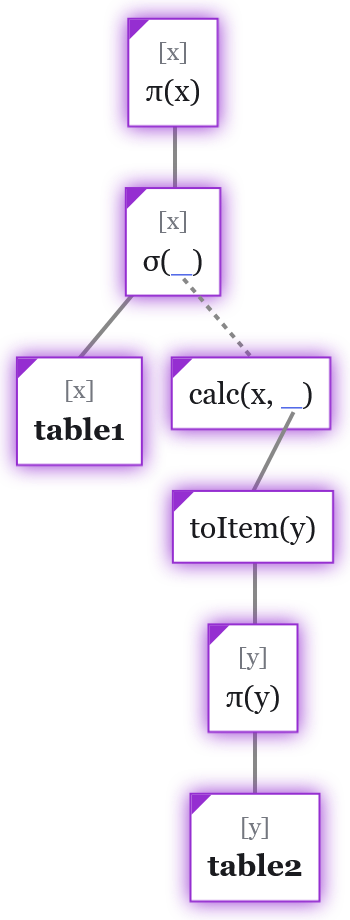
\includegraphics[width=100pt]{img/tree-naive-subquery.png}
    \end{subfigure}
    
    \caption{A subquery can be expressed as a \texttt{calculation} with a \texttt{projection} as an argument.}
    \label{fig:naive-subquery}
\end{figure}

The rest of the full-fledged item operators are data sources, and the \texttt{mapToItem} operator converts tuples to items. It selects the \texttt{key} attribute from each tuple. If the \texttt{key} is the \textit{allAttrs symbol *}, the whole tuple is treated as the new item.

Tuple operators include the well-known \texttt{selection}, \texttt{projection}, \texttt{join}, \\\texttt{cartesianProduct}, and \texttt{orderBy}. \texttt{Join} may include multiple conditions, in which case they must all be satisfied for the two source tuples to be joined. Multiple separated conditions make it easier for the optimizer to recognize certain opportunities. It is also possible to not specify any condition at all and to use the \texttt{join} operator solely for its \texttt{leftOuter} or \texttt{rightOuter} properties.

\texttt{ProjectionIndex} adds a new attribute to each tuple that tracks its ordinal number. \texttt{ProjectionConcat} could be also called \texttt{depend-join}. It is similar to \texttt{join}, in that it joins \texttt{source} tuples to \texttt{mapping} tuples. For each \texttt{source} tuple, the \texttt{mapping} stream is reevaluated, and each of its tuples is joined to the \texttt{source} tuple. The \texttt{mapping} may depend on the context of the \texttt{source} stream. In terms of SQL, the \texttt{projectionConcat} operator can be utilized in correlated subqueries in the \texttt{SELECT} or \texttt{WHERE} clause, or in \texttt{LATERAL JOIN}.

\begin{figure}[htpb]
    \begin{subfigure}[b]{\textwidth}
    \begin{tcolorbox}[colback=white, colframe=black, boxrule=1pt, arc=0pt]
        \begin{minted}[fontsize=\small]{sql}
SELECT x FROM table1
WHERE x < (
  SELECT y FROM table2
)
        \end{minted}
    \end{tcolorbox}
    \end{subfigure}
    
    \medskip
    
    \begin{subfigure}[b]{\textwidth}
        \centering
        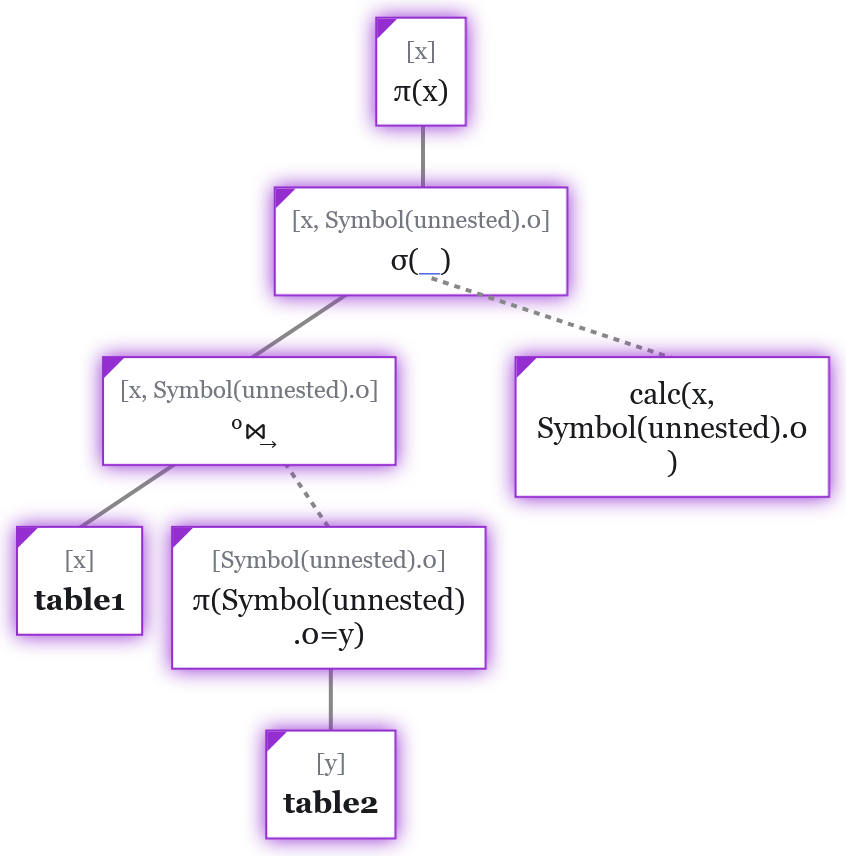
\includegraphics[width=220pt]{img/tree-projconcat-subquery.png}
    \end{subfigure}
    
    \caption{The same query as in figure \ref{fig:naive-subquery}, but the optimizer converted the nested \texttt{projection} to an outer \texttt{projectionConcat}. Note that this is not yet fully optimized. Because the nested \texttt{projection} does not depend on \textbf{table1} context, the \texttt{projectionConcat} can be further converted to a left \texttt{join}.}
\end{figure}

The \texttt{distinct} operator filters out duplicate tuples. The duplicates are decided based on \texttt{attributes}. Similarly to \texttt{mapToItem}, \texttt{attributes} may be the \textit{allAttrs symbol *}. The \texttt{mapFromItem} operator converts an item to a tuple with one attribute named \texttt{key}, which contains the original item. It is not possible to interpret the original item as a tuple.

\texttt{GroupBy} groups \texttt{source} values into partitions based on \texttt{keys}. Each partition is then processed by \texttt{aggregateCall} operators in \texttt{aggs}. Each \texttt{aggregateCall} may contain additional operators that preprocess the partition stream before it is aggregated, for example, when the aggregate requires certain ordering or filtering.

\begin{figure}[htpb]
    \begin{subfigure}[b]{\textwidth}
    \begin{tcolorbox}[colback=white, colframe=black, boxrule=1pt, arc=0pt]
        \begin{minted}[fontsize=\small]{sql}
SELECT
  count(id) FILTER (WHERE sex = 'M') AS men,
  count(id) FILTER (WHERE sex = 'F') AS women,
  collect(DISTINCT id ORDER BY id) AS all_ids
FROM sales
GROUP BY brand
        \end{minted}
    \end{tcolorbox}
    \end{subfigure}
    
    \medskip
    
    \begin{subfigure}[b]{\textwidth}
        \centering
        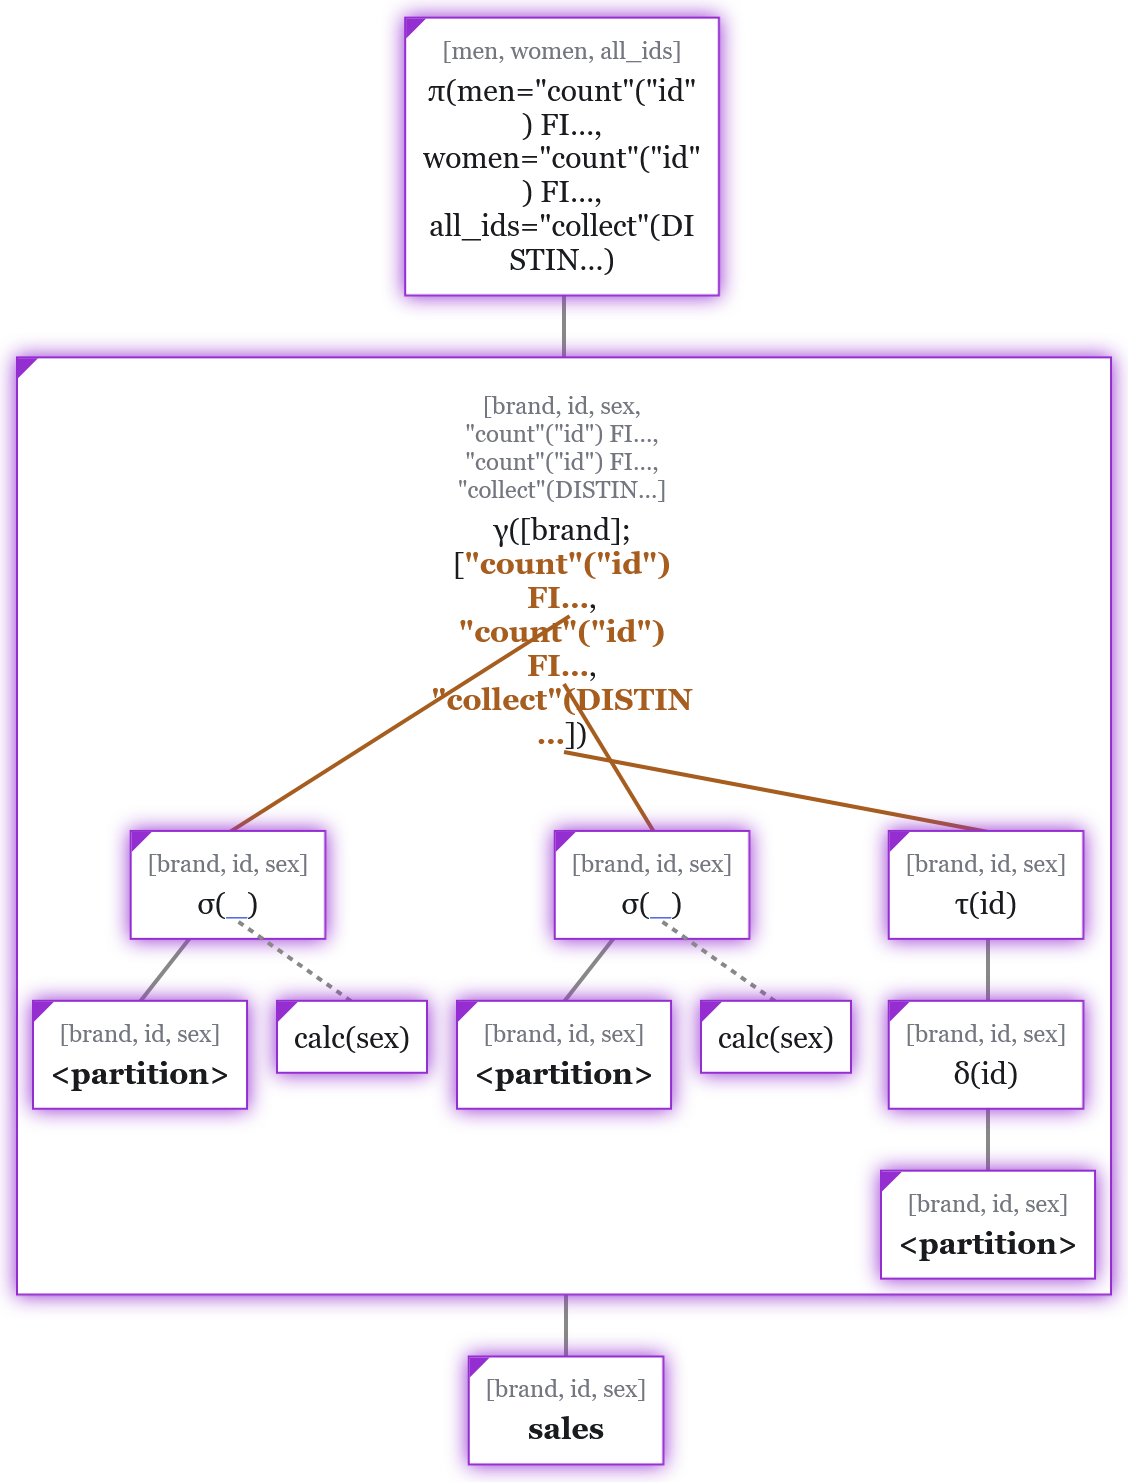
\includegraphics[width=380pt]{img/tree-groupby.png}
    \end{subfigure}
    
    \caption{Example of a complex SQL aggregation. The \texttt{FILTER} clause is defined in SQL:2003 as an optional feature. It is implemented in PostgreSQL and SQLite.}
\end{figure}

The \texttt{Recursion} operator is a self-join repeated up to \texttt{max} times. Its \texttt{condition} can access each \texttt{source} attribute as a pair of an array of accumulated values and the potential next value. The query executor is required to execute the recursion using breadth-first search, so that the shortest values are generated first.

\pagebreak

In order to properly apply indices, there are two specialized operators. \texttt{Index\-Scan} replaces a \texttt{tupleSource} or an \texttt{itemSource} paired with a \texttt{mapFromItem}. It contains an \texttt{access} \texttt{calculation}, which selects relevant items from the underlying data source. The self-join implementation of \texttt{recursion} does not leave any opportunity for indices, so it may be more efficient to use the \texttt{indexedRecursion} operator, which acts as a self-depend-join.

Among the universal operators, which can process both tuples and items, belong the classic set operators like \texttt{union}, \texttt{intersection}, and \texttt{difference}. The \texttt{limit} operator allows only a set amount of results. \texttt{NullSource} is a data source that emits only one empty item.

\begin{figure}[htpb]
    \begin{subfigure}[b]{\textwidth}
    \begin{tcolorbox}[colback=white, colframe=black, boxrule=1pt, arc=0pt]
        \begin{minted}[fontsize=\small]{sql}
SELECT 1 AS one
        \end{minted}
    \end{tcolorbox}
    \end{subfigure}
    
    \medskip
    
    \begin{subfigure}[b]{\textwidth}
        \centering
        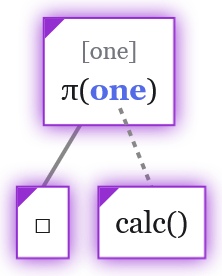
\includegraphics[width=70pt]{img/tree-null-source.png}
    \end{subfigure}
    
    \caption{One possible application for the \texttt{nullSource} operator.}
\end{figure}

Finally, there are two operators used only by XQuery. The \texttt{projectionSize} operator adds a new attribute to each tuple that contains the cardinality of the tuple stream. \texttt{TreeJoin} is a utility operator, which combines \texttt{projectionConcat}, \texttt{projectionIndex} and \texttt{projectionSize}. It is used for path steps like \mintinline{xquery}{a/b/c}. For each step in the path, XQuery must provide a context containing the current item, its position, and the total item count. One notable difference between \texttt{treeStep} and \texttt{projectionConcat} is that \texttt{expr} is a \texttt{calculation} instead of a tuple operator.

\begin{figure}[htpb]
    \begin{subfigure}[b]{\textwidth}
    \begin{tcolorbox}[colback=white, colframe=black, boxrule=1pt, arc=0pt]
        \begin{minted}[fontsize=\small]{cypher}
MATCH ()-[path *2]->()
RETURN path
        \end{minted}
    \end{tcolorbox}
    \end{subfigure}

    \medskip
    
    \begin{subfigure}{\textwidth}
        \centering
        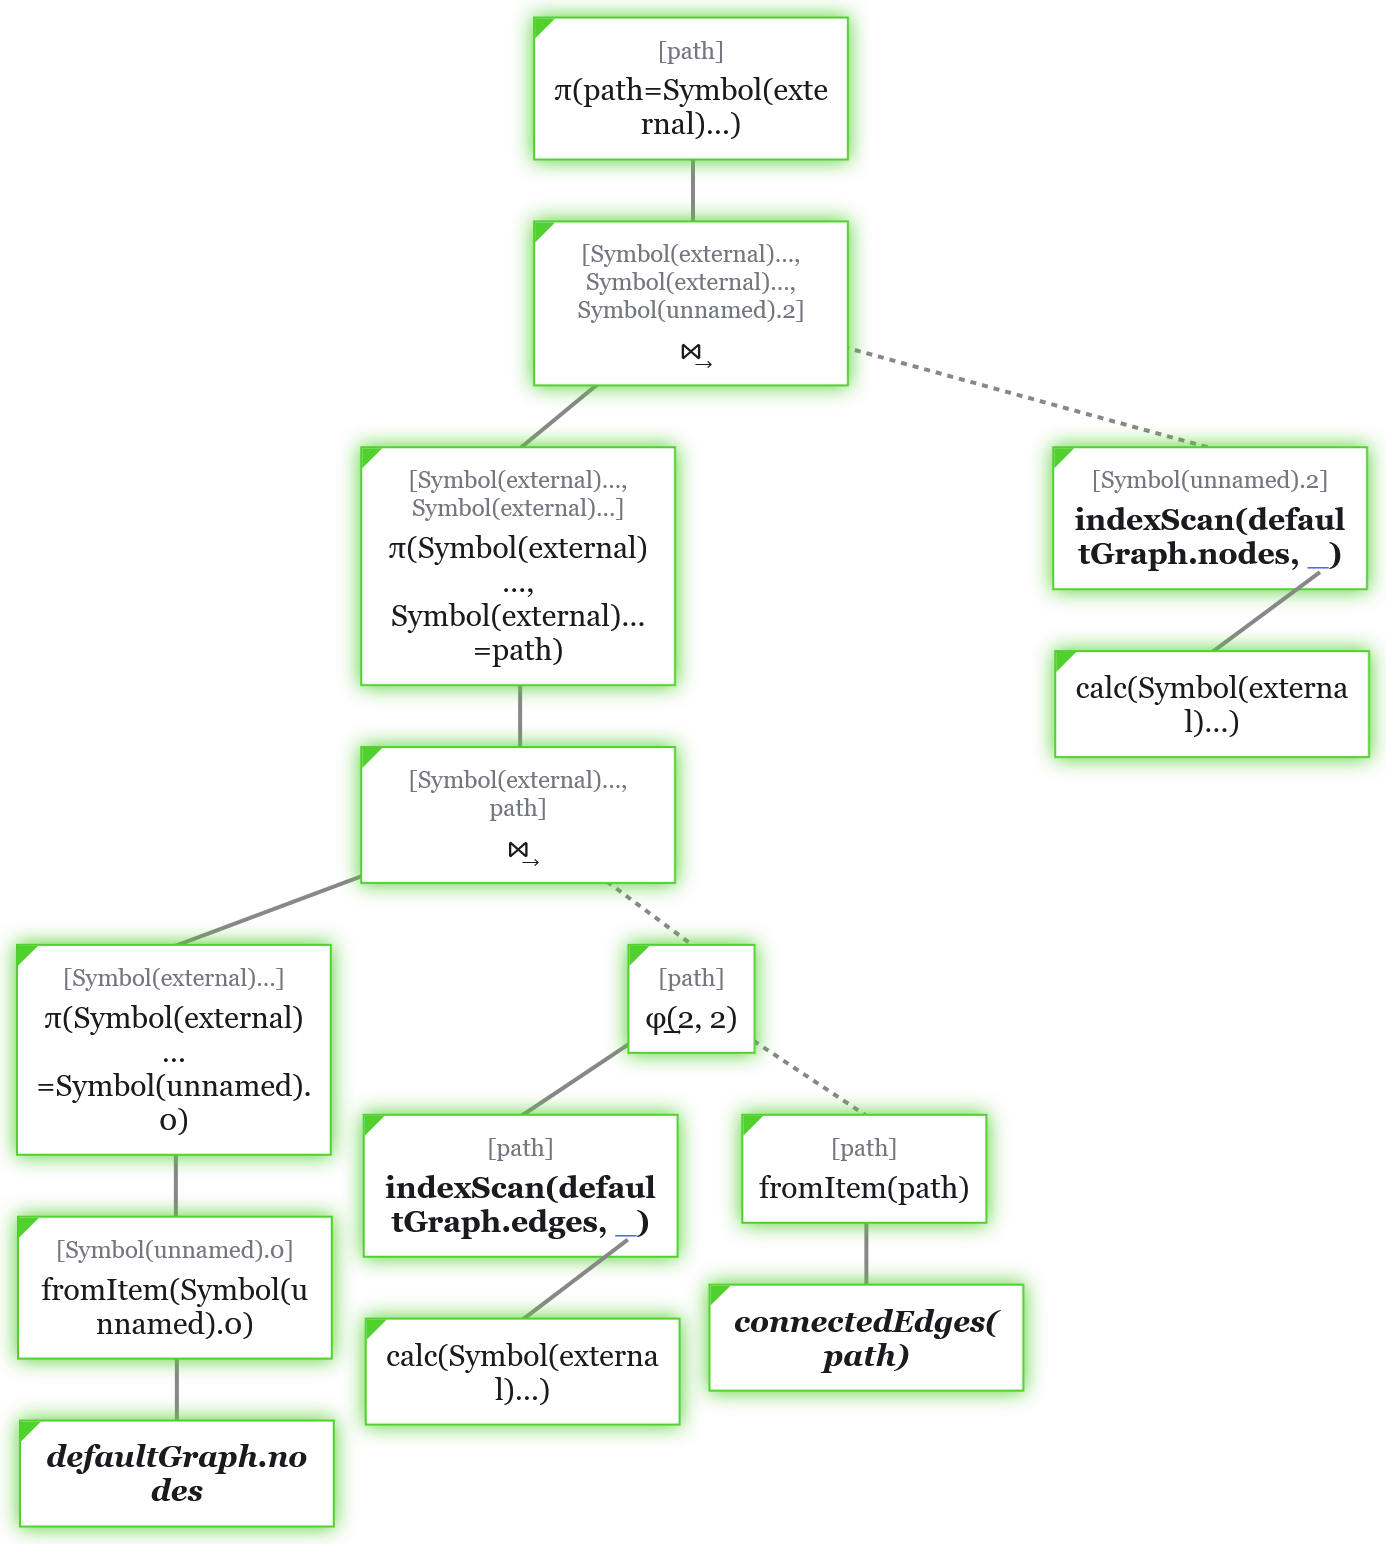
\includegraphics[width=\textwidth]{img/tree-indexed-recursion.png}
    \end{subfigure}
    
    \caption{This cypher query first selects all nodes from a graph. It then selects all of their outgoing edges using an \texttt{indexScan}. These edges are recursively expanded into two-segment paths with the \texttt{indexedRecursion} operator. Finally, another \texttt{indexScan} selects the end nodes of the paths.}
    \label{fig:tree-indexed-recursion}
\end{figure}